\section{Theorie}
\label{sec:Theorie}

Als ein gekoppeltes Schwingsystem sind zwei durch eine Feder verbundene Fadenpendel schwer zu untersuchen sind.
Es wird daher auf elektrische Schwingkreise zurückgegriffen, da Frequenz und Amplitude dabei leichter zu bestimmen sind.

\subsection {Verhalten kapazitiv gekoppelter Schwingkreise}

Es werden zwei identische Schwingkreise betrachtet, die durch eine Kapazität $C_{K}$ miteinander verbunden sind.

\begin{figure} 
    \centering
    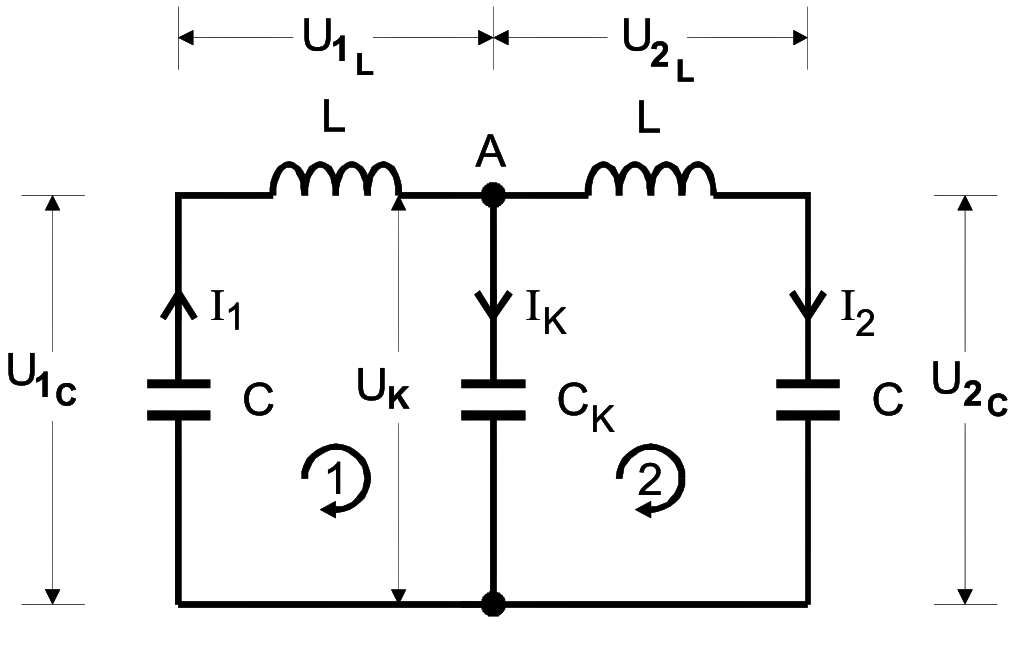
\includegraphics[width=8cm] {pictures/prinzipschaltbild.png} \cite{v355} 
    \caption{Schaltung kapazitiv gekoppelter Schwingkreise}
    \label{fig:prinzipschaltbild}
\end{figure} 

